\documentclass{beamer}
\usepackage[english]{babel}
\usepackage{url}
\usepackage{listings}
\usepackage{adjustbox}
\usepackage{chronology}
\newcommand{\LO}{$\mathcal{L}_0$}

% \usepackage{sfmath}
% \usepackage{lxfonts}
% \usepackage{mathdesign}
\usepackage{unicode-math}
% \setmathfont{lmmath-regular.otf}
% \setmathfont{lmmath-regular.otf}
% \setmathfont{Asana-Math.otf}
% \setmathfont{xits-math.otf}


% Graphics
\usepackage{graphicx}
% \usepackage{tikz}
% \usetikzlibrary{matrix, calc, arrows, snakes}

% Figures
\usepackage{caption}
\captionsetup{labelformat=empty,labelsep=none}

% Font
\usepackage{microtype}
% \usepackage[scaled]{beramono}
\usepackage{fontspec,xunicode}
\newfontfamily\sbmyriad{Myriad Pro Semibold}
\setsansfont{Myriad Pro}
\setmonofont{Myriad Pro}
\setbeamerfont{title}{family=\sbmyriad}
\setbeamerfont{frametitle}{family=\bf}


% Beamer theme settings
\usecolortheme{seagull}
\setbeamertemplate{itemize item}{\raisebox{0.8mm}{\rule{1.2mm}{1.2mm}}}
\usenavigationsymbolstemplate{} % no navigation buttons

\lstdefinelanguage{L0}
{keywords={fun,if,then,else,loop,do,map,reduce,filter,scan,redomap,mapT,reduceT,filterT,scanT,redomapT,transpose,reshape,iota,replicate,let},%
sensitive=true,%
comment=[l]{//},%
string=[b]",%
string=[b]'%
}

\lstset{
  language=L0
}

\title{Master's thesis defence}
\subtitle{Exploiting functional invariants to optimise parallelism:\\ A dataflow approach}
\author{Troels Henriksen}
\date{21. February 2014}
\institute{Computer Science\\
  University of Copenhagen}

\begin{document}
% Welcome
% Both a defence and this is what I do
\frame{\titlepage}

% % Nice diagram showing how the talk will progress
% \begin{frame}
%   \frametitle{Agenda}
%   \tableofcontents
% \end{frame}

\begin{frame}
  \frametitle{Free lunches}

  \begin{itemize}
  \item Moores law still in effect, and will be for a while..
  \item ... but we no longer get many increases in sequential
    performances.
  \item Modern performance increases are in the form of parallelism.
  \item The most parallel machines are massively parallel vector
    processors, with commodity GPUs being particularly interesting due
    to their ubiquity.
  \end{itemize}

\end{frame}

\begin{frame}
  \frametitle{GPGPU}

  \begin{itemize}
  \item GPUs were popularised in the 90s for graphics processing.
  \item Graphics is inherently parallel, so for cost reasons, the GPU
    hardware was very parallel as well.
  \item In roughly 2006, GPGPU began to take off with CUDA and then
    OpenCL.
  \item GPGPU is now widespread, but still very difficult.
  \end{itemize}
\end{frame}

\begin{frame}
  \frametitle{GPGPU, continued}

  \begin{itemize}
  \item OpenCL and CUDA both very low-level.
  \item No modularisation if you want performance.
  \item Libraries can contain optimised primitives... modular
    performance still tricky.
  \item So we need a language.
  \end{itemize}
\end{frame}

\begin{frame}
  \frametitle{Language design}

  \begin{itemize}
  \item Three real-world financial computational kernels served to
    guide the design.  Two central questions:
    \begin{itemize}
    \item \textbf{What is the simplest language that permits a
        relatively straightforward translation of the financial
        programs, while still expressing algorithm invariants that
        enable the generation of efficient parallel code?}
    \item \textbf{What compiler optimizations would result in efficiency
        comparable to code hand-tuned for the specific hardware?}
    \end{itemize}
  \item We ended up on a functional language, \LO{}, supporting nested
    parallelism on regular arrays.
  \item Fusion is one of the most important optimisations.  ``Heroic
    Effort'' in an imperative language, but ``easy'' in a functional
    setting.
  \end{itemize}
\end{frame}

\begin{frame}[fragile]
  \frametitle{Hello, World!}

\begin{lstlisting}
fun fact(int n) =
  if n = 0 then 1
           else n * fact(n-1)
\end{lstlisting}

\begin{lstlisting}
fun hofact(int n) =
  reduce(op *, 1, iota(n))
\end{lstlisting}

We have the following second-order array combinators (SOACs):
\textbf{reduce}, \textbf{map}, \textbf{scan}, \textbf{filter} and
\textbf{redomap}.

\end{frame}

\begin{frame}[fragile]
  \frametitle{In-place updates}

  The innermost part of a parallel loop may be a sequential
  computation.

\begin{lstlisting}
fun [int] fib(int n) =
  // Create "empty" array.
  let arr = iota(n) in
  // Fill array with Fibonacci numbers.
  loop (arr) =
    for i < n-2 do
      let arr[i+2] = arr[i] + arr[i+1]
      in arr
  in arr
\end{lstlisting}

Runs in $O(n^{2})$ if the array update is not in-place!  Permitting
mutation of the array allows an asymptotic improvement to $O(n)$.

\end{frame}

\begin{frame}[fragile]
  \frametitle{Uniqueness types}

  A \textit{unique-typed function argument} is guaranteed not to be
  referenced again on any execution path following the function call.

\begin{lstlisting}
  fun *[int] modify(*[int] a, int i, int x) =
    let a[i] <- a[i] + x in
    a
\end{lstlisting}

This runs in $O(1)$.

The return type is also unique -- this means that there are no other
references to the value.
\end{frame}

\begin{frame}
\frametitle{\textbf{redomap}}
\end{frame}

\begin{frame}
\frametitle{Tupleless SOACs}
\end{frame}

\begin{frame}
\frametitle{Fusion on dataflow graph}

\end{frame}

\begin{frame}[fragile]
\frametitle{Fusion example, continued}

We will try to fuse the following program.

\begin{lstlisting}
let {x1} = mapT(h1, x2) in
let {y1,y2,y3} = mapT(f1, x1, x2) in
let {z1,z2} = mapT(f2, y1, y2) in
let {q1,q2} = mapT(g,y3,z1,y2,y3) in
{mapT(h, q1, q2, z2, y1, y3),
 mapT(h2, x2)}
\end{lstlisting}

Note that some outputs are used multiple times as inputs to different
SOACs.

\end{frame}

\begin{frame}[t]
\frametitle{Fusion example, continued}

\begin{center}
\begin{columns}[t]
  \begin{column}{0.5\textwidth}
    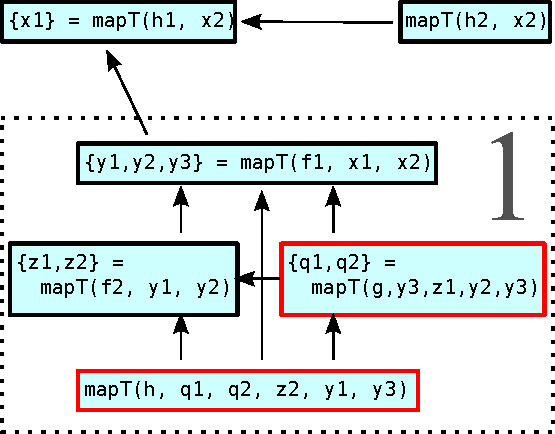
\includegraphics[width=4cm]{img/fusion-1.pdf}
    \vspace{1cm}
    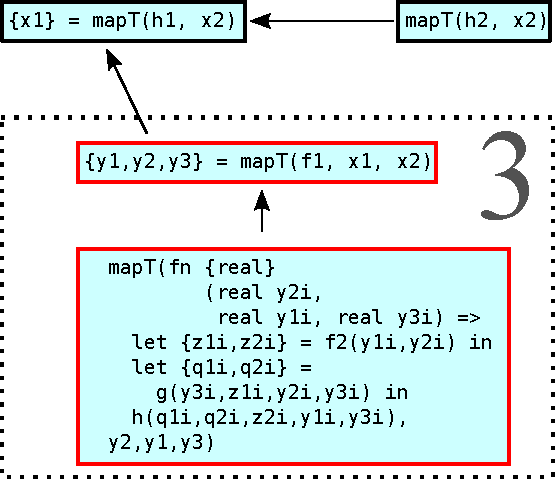
\includegraphics[width=4cm]{img/fusion-3.pdf}
  \end{column}

  \begin{column}{0.5\textwidth}
    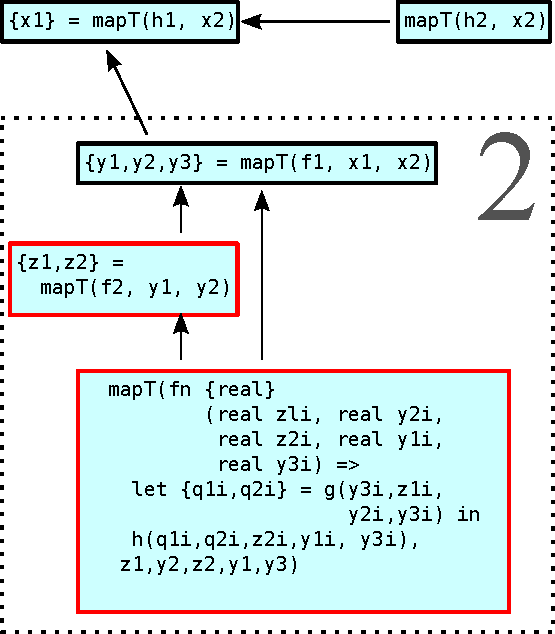
\includegraphics[width=4cm]{img/fusion-2.pdf}
    \vspace{1cm}
    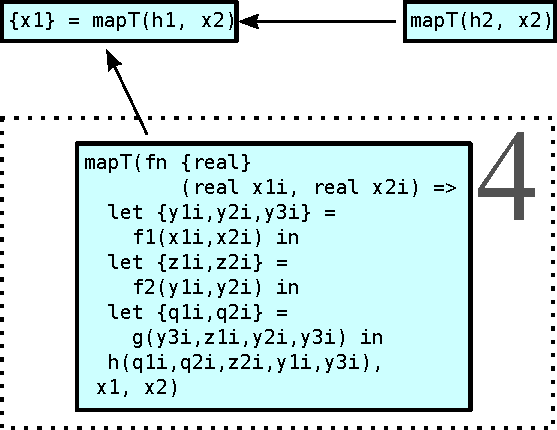
\includegraphics[width=4cm]{img/fusion-4.pdf}
  \end{column}
\end{columns}
\end{center}

\end{frame}

\end{document}

%%% Local Variables:
%%% mode: latex
%%% TeX-engine: luatex
%%% End:
